\documentclass[10pt]{beamer}

\newcommand{\lectnum}{L04}
\newcommand{\lecttitle}{Neural Networks}

\usepackage{amsmath, amssymb, graphicx}
\usepackage[]{algorithm2e}
\usepackage{pdfpages}
\usepackage{bm}
\usepackage{relsize}
\usepackage[british]{babel}
\usepackage{tikz,tikzsymbols}
\usepackage{pgfplots}
\pgfplotsset{compat=1.17}
\usepackage{listings}
\lstset{language=Python, basicstyle=\ttfamily\scriptsize,
  keywordstyle=\bfseries\color{blue!60!black},
  commentstyle=\color{gray}, stringstyle=\color{red!60!black},
  showstringspaces=false, columns=flexible, keepspaces=true,
  frame=single, rulecolor=\color{gray!40}, backgroundcolor=\color{gray!5},
  xleftmargin=2pt, xrightmargin=2pt}
\usepackage{hyperref}
\usepackage{cancel}
\usepackage{caption,subcaption}
\usepackage{adjustbox}
\usepackage{overpic}
\usepackage[UKenglish]{isodate}

\usetikzlibrary{arrows,decorations.markings,positioning}

\newcommand{\bs}{\boldsymbol}


\hypersetup{colorlinks,linkcolor=,urlcolor=blue}
\newenvironment{titledslide}[1]{\begin{frame}\frametitle{#1}}{\end{frame}}

\mode<presentation>{\setbeamercovered{transparent}}

\setbeamertemplate{sidebar right}{}
\setbeamertemplate{footline}{%
\hfill\usebeamertemplate***{navigation symbols}
\hspace{0.4cm}\lectnum: \insertframenumber{}/\inserttotalframenumber \hspace*{0.4cm}}

\author{Mengyan Zhang}

\title{COMS20018, Introduction to AI:\\ \vspace{5pt} \lecttitle}

\institute{School of Computer Science\\University of Bristol}
\date{29th September 2026}

%%%%%%%%%%%%%%%%%%%%%%%%%%%%%%%%%%%%%%%%%%%%%%%%%%%%%%%%%%%%%%%%%%%%%%

\begin{document}
%%%%%%%%%%%%%%%%%%%%%%%%%%%%%%%%%%%%%%%%%%%%%%%%%%%%%%%%%%%%%%%%%%%%%%

\begin{frame}[fragile]
  \begin{tikzpicture}[remember picture, overlay]
    \node[anchor=north west, xshift=0.4cm, yshift=-0.4cm] at (current page.north west)
      {
\includegraphics[width=3.4cm]{figures/uob_logo.png}};
  \end{tikzpicture}
  \titlepage
\end{frame}
%%%%%%%%%%%%%%%%%%%%%%%%%%%%%%%%%%%%%%%%%%%%%%%%%%%%%%%%%%%%%%%%%%%%%%
\begin{frame}[fragile]
\frametitle{Agenda}

  \begin{itemize}
  \item Feed-forward network functions: A two-layer network \hfill
  \item Training a network \hfill
    \begin{itemize}
    \item A nonconvex loss: global vs.\ local minima, saddle points
    \item (Mini-batch) SGD
    \end{itemize}
  \item Chain rule and error backpropagation \hfill
    \begin{itemize}
    \item Computing gradients efficiently
    \item Autograd and training loops in PyTorch
    \end{itemize}
  \end{itemize}

\end{frame}
%%%%%%%%%%%%%%%%%%%%%%%%%%%%%%%%%%%%%%%%%%%%%%%%%%%%%%%%%%%%%%%%%%%%%%
\begin{frame}[fragile]
\frametitle{A two-layer network (1/3): the hidden layer}

\begin{columns}[c]
\begin{column}{0.42\textwidth}
\centerline{\begin{tikzpicture}
  \node[anchor=south west,inner sep=0] (img) at (0,0)
    {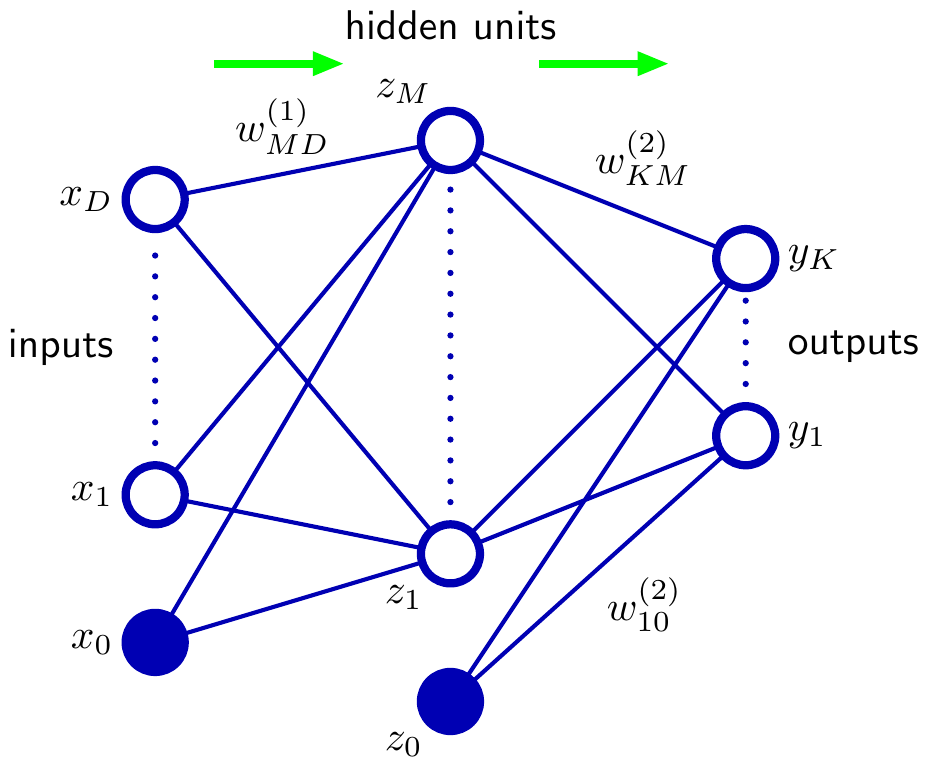
\includegraphics[width=\linewidth]{figures/prml_fig5_1.png}};
  \begin{scope}[x={(img.south east)},y={(img.north west)}]
    \fill[white,opacity=0.7] (0.555,0) rectangle (1,0.935);
    \fill[white,opacity=0.7] (0.36,0) rectangle (0.555,0.12);
    \draw[blue!70!black,thick,rounded corners=6pt]
      (0.005,0.105) -- (0.345,0.105) -- (0.345,0.185) -- (0.545,0.185)
      -- (0.545,0.925) -- (0.005,0.925) -- cycle;
  \end{scope}
\end{tikzpicture}}

{\scriptsize Bishop, \emph{PRML} (2006), Fig.\ 5.1: filled nodes
$x_0{=}z_0{=}1$ carry the biases.}
\end{column}
\begin{column}{0.55\textwidth}
\begin{itemize}
\item Input $\bs{x} = (x_1,\dots,x_D)^\top$, plus a bias $x_0{=}1$.
\item Each of the $M$ \textbf{hidden units} takes a weighted sum of the
  inputs, then applies a \textit{differentiable, nonlinear} activation function $h$:
\[
{\color{blue!70!black}a_j = \sum_{i=0}^{D} w^{(1)}_{ji}\, x_i, \qquad z_j = h(a_j)}
\]
\end{itemize}
\end{column}
\end{columns}

\end{frame}
%%%%%%%%%%%%%%%%%%%%%%%%%%%%%%%%%%%%%%%%%%%%%%%%%%%%%%%%%%%%%%%%%%%%%%
\begin{frame}[fragile]
\frametitle{A two-layer network (2/3): the output layer}

\begin{columns}[c]
\begin{column}{0.42\textwidth}
\centerline{\begin{tikzpicture}
  \node[anchor=south west,inner sep=0] (img) at (0,0)
    {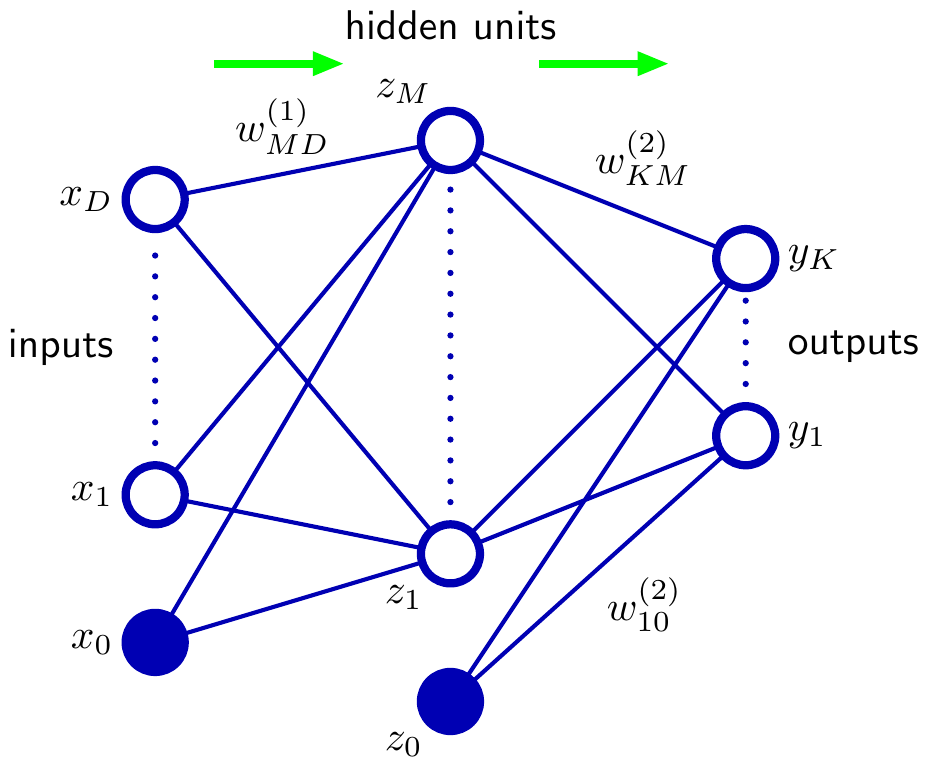
\includegraphics[width=\linewidth]{figures/prml_fig5_1.png}};
  \begin{scope}[x={(img.south east)},y={(img.north west)}]
    \fill[white,opacity=0.7] (0,0) rectangle (0.37,0.935);
    \draw[orange!85!black,thick,rounded corners=6pt] (0.38,0.005) rectangle (0.995,0.925);
  \end{scope}
\end{tikzpicture}}

{\scriptsize Bishop, \emph{PRML} (2006), Fig.\ 5.1: filled nodes
$x_0{=}z_0{=}1$ carry the biases.}
\end{column}
\begin{column}{0.55\textwidth}
\begin{itemize}
\item The hidden units (plus a bias $z_0{=}1$) feed the outputs
  $y_1,\dots,y_K$:
\[
{\color{orange!85!black}y_k = f\Bigl(\sum_{j=0}^{M} w^{(2)}_{kj}\, z_j\Bigr)}
\]
\item $K$ outputs: $K{=}1$ for a scalar target; $K{>}1$ for a
  vector target $\bs{t}\in\mathbb{R}^K$
\item Output activation $f$: identity (regression), sigmoid $\sigma$
  (binary classification), softmax (multiclass classification), etc. 
\end{itemize}
\end{column}
\end{columns}

\end{frame}
%%%%%%%%%%%%%%%%%%%%%%%%%%%%%%%%%%%%%%%%%%%%%%%%%%%%%%%%%%%%%%%%%%%%%%
\begin{frame}[fragile]
\frametitle{A two-layer network (3/3): putting it together}

\begin{columns}[c]
\begin{column}{0.42\textwidth}
\centerline{\begin{tikzpicture}
  \node[anchor=south west,inner sep=0] (img) at (0,0)
    {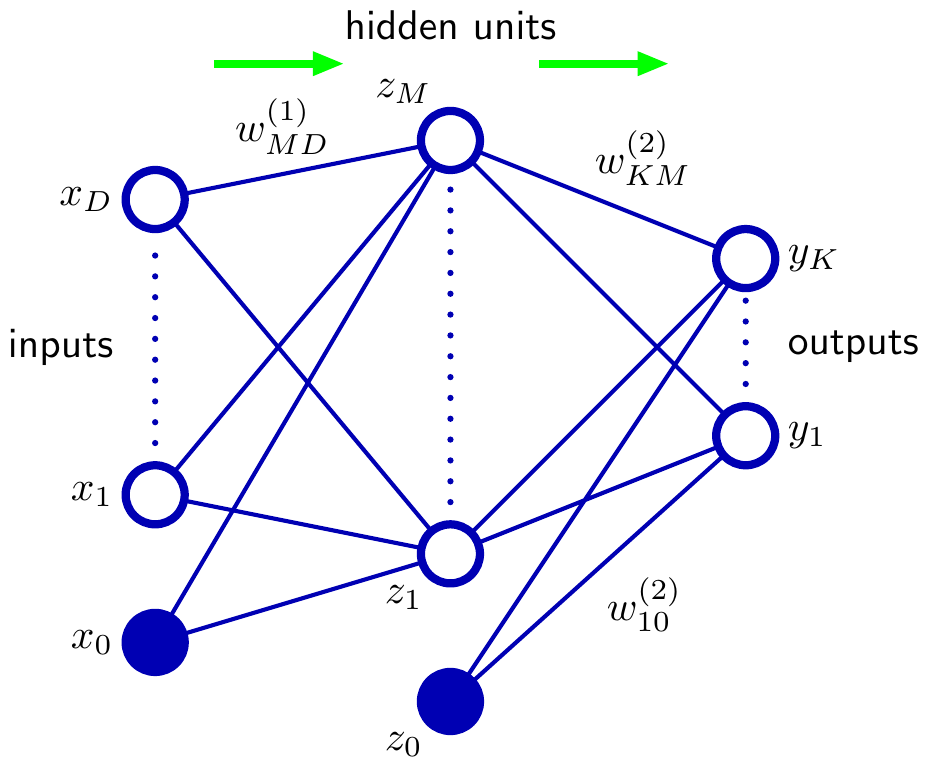
\includegraphics[width=\linewidth]{figures/prml_fig5_1.png}};
\end{tikzpicture}}

{\scriptsize Bishop, \emph{PRML} (2006), Fig.\ 5.1: filled nodes
$x_0{=}z_0{=}1$ carry the biases.}
\end{column}
\begin{column}{0.55\textwidth}
\begin{itemize}
\item Substitute the {\color{blue!70!black}hidden layer} into the {\color{orange!85!black}output
  layer}.
\item[$\Rightarrow$] One differentiable function of \emph{all} weights
  $\bs{w} = (w^{(1)}_{ji}, w^{(2)}_{kj})$; evaluating it left to right is
  \textbf{forward propagation}.
\end{itemize}
\end{column}
\end{columns}

\vspace{4pt}
\[
y_k(\bs{x},\bs{w}) = {\color{orange!85!black}f\Bigl(\sum_{j=1}^{M} w^{(2)}_{kj}\,
{\color{blue!70!black}h\Bigl(\sum_{i=1}^{D} w^{(1)}_{ji}x_i + w^{(1)}_{j0}\Bigr)} +
w^{(2)}_{k0}\Bigr)}
\]

\end{frame}
%%%%%%%%%%%%%%%%%%%%%%%%%%%%%%%%%%%%%%%%%%%%%%%%%%%%%%%%%%%%%%%%%%%%%%
\begin{frame}[fragile]
\frametitle{Activation functions: why the nonlinearity matters}

\begin{columns}[c]
\begin{column}{0.43\textwidth}
\centerline{\resizebox{\linewidth}{!}{%
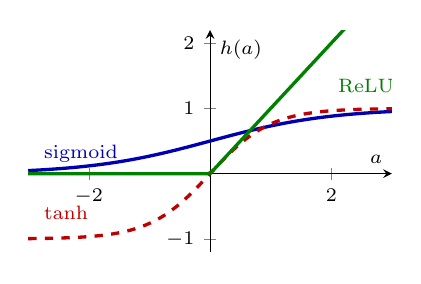
\begin{tikzpicture}
\begin{axis}[
  width=6.2cm, height=4.4cm,
  xlabel={$a$}, ylabel={$h(a)$},
  xmin=-3, xmax=3, ymin=-1.2, ymax=2.2,
  axis lines=middle, samples=100, domain=-3:3,
  label style={font=\scriptsize}, tick label style={font=\scriptsize},
]
\addplot[blue!70!black, very thick] {1/(1+exp(-x))};
\addplot[red!75!black, very thick, dashed] {tanh(x)};
\addplot[green!50!black, very thick] {max(0,x)};
\node[font=\scriptsize, text=blue!70!black, anchor=west] at (axis cs:-2.9,0.3) {sigmoid};
\node[font=\scriptsize, text=red!75!black, anchor=west] at (axis cs:-2.9,-0.6) {$\tanh$};
\node[font=\scriptsize, text=green!50!black, anchor=west] at (axis cs:1.95,1.35) {ReLU};
\end{axis}
\end{tikzpicture}}}
\end{column}
\begin{column}{0.54\textwidth}
\small
\begin{itemize}
\item Common choices for $h$:
  \begin{itemize}
  \item \textbf{sigmoid}, $\sigma(a) = \dfrac{1}{1+e^{-a}}$: output in
    $(0,1)$
  \item \textbf{tanh}, $\tanh(a) = \dfrac{e^{a}-e^{-a}}{e^{a}+e^{-a}}$:
    output in $(-1,1)$, a rescaled sigmoid centred at 0
  \item \textbf{ReLU}, $\max(0,a)$: cheap, its slope
    doesn't vanish for $a>0$
  \end{itemize}
% \item \textbf{Universal approximation}: with enough hidden units $M$, a
%   two-layer network can approximate any continuous function
%   arbitrarily well (Bishop \S5.1).
\item[$\Rightarrow$] Stack more layers $\Rightarrow$ a \textbf{deep}
  network: richer, adaptive basis functions.
\end{itemize}
\end{column}
\end{columns}

\vspace{6pt}
\begin{itemize}
\item Why nonlinear (for hidden units)? If $h$ were linear, the two
  layers would collapse into a single linear layer
\end{itemize}

\end{frame}
%%%%%%%%%%%%%%%%%%%%%%%%%%%%%%%%%%%%%%%%%%%%%%%%%%%%%%%%%%%%%%%%%%%%%%
% \begin{frame}[fragile]
% \frametitle{Learned basis functions in action}

% \begin{columns}[c]
% \begin{column}{0.52\textwidth}
% \centerline{\includegraphics[width=\linewidth]{figures/prml_fig5_3.png}}

% \vspace{2pt}
% {\scriptsize Bishop, \emph{PRML} (2006), Fig.\ 5.3.}
% \end{column}
% \begin{column}{0.45\textwidth}
% \begin{itemize}
% \item A two-layer network with $M{=}3$ $\tanh$ hidden units and a linear
%   output, fitted to $N{=}50$ points ({\color{blue}blue}) from (a) $x^2$,
%   (b) $\sin x$, (c) $|x|$, (d) a step.
% \item {\color{red}Red}: the network output. Dashed: the three hidden
%   units $z_j$.
% \item[$\Rightarrow$] Same architecture, different learned weights
%   $\Rightarrow$ different basis functions, each tailored to the data.
% \end{itemize}
% \end{column}
% \end{columns}

% \end{frame}
%%%%%%%%%%%%%%%%%%%%%%%%%%%%%%%%%%%%%%%%%%%%%%%%%%%%%%%%%%%%%%%%%%%%%%
\begin{frame}[fragile]
\frametitle{Parameter optimisation}

\begin{itemize}
\item Define a loss function over the training set, e.g.\
  sum-of-squares (regression) or cross-entropy (classification), now as a
  function of \emph{all} the network's weights $\bs{w}$.
\end{itemize}

\begin{itemize}
\item Least squares was \emph{quadratic} (closed form); logistic regression had no closed form, but the loss was convex.
\item For typical multilayer neural networks, $L(\bs{w})$ is generally \textbf{nonconvex} in $\bs{w}$ -  No closed-form solution; search for a good
  $\bs{w}$ iteratively
\end{itemize}

\vspace{4pt}
\centerline{%
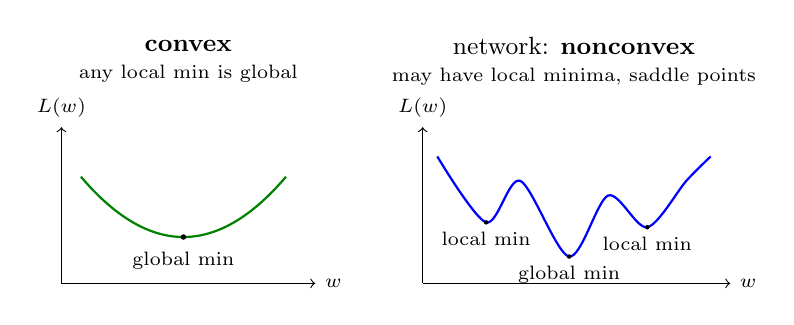
\begin{tikzpicture}[scale=0.62,every node/.style={font=\scriptsize}]
  % L03: convex
  \draw[->] (0,0) -- (5.2,0) node[right]{$w$};
  \draw[->] (0,0) -- (0,3.2) node[above]{$L(w)$};
  \draw[thick,green!50!black,domain=0.4:4.6,samples=60] plot (\x,{0.28*(\x-2.5)^2+0.95});
  \fill (2.5,0.95) circle (1.6pt) node[below=2pt]{global min};
  \node[font=\small,align=center] at (2.6,4.55) {\textbf{convex}\\[-1pt]{\scriptsize any local min is global}};
  % network: nonconvex
  \begin{scope}[xshift=7.4cm]
  \draw[->] (0,0) -- (6.3,0) node[right]{$w$};
  \draw[->] (0,0) -- (0,3.2) node[above]{$L(w)$};
  \draw[thick,blue] plot[smooth] coordinates
    {(0.3,2.6)(1.3,1.25)(2.0,2.1)(3.0,0.55)(3.8,1.8)(4.6,1.15)(5.4,2.1)(5.9,2.6)};
  \fill (1.3,1.25) circle (1.3pt) node[below]{local min};
  \fill (3.0,0.55) circle (1.3pt) node[below]{global min};
  \fill (4.6,1.15) circle (1.3pt) node[below]{local min};
  \node[font=\small,align=center] at (3.1,4.55) {network: \textbf{nonconvex}\\[-1pt]{\scriptsize may have local minima, saddle points}};
  \end{scope}
\end{tikzpicture}}

\end{frame}
%%%%%%%%%%%%%%%%%%%%%%%%%%%%%%%%%%%%%%%%%%%%%%%%%%%%%%%%%%%%%%%%%%%%%%
\begin{frame}[fragile]
\frametitle{(S)GD on a neural network: what changes?}

\begin{columns}[c]
\begin{column}{0.57\textwidth}
\small
\begin{itemize}
\item A stationary point, $\nabla L = 0$, can now be a local minimum, the
  global minimum, or a \textbf{saddle point}; different initialisations can
  lead to different solutions.
\item In practice: \textbf{mini-batch} SGD, averaging $\nabla L_n$
  over a small batch (e.g.\ 32--256 examples), balancing noise vs.\
  speed.
\item[$\Rightarrow$] Modern refinements: \textbf{momentum}, adaptive
  step sizes (\textbf{Adam}); see Goodfellow et al., Ch.\,8.
\end{itemize}
\end{column}
\begin{column}{0.4\textwidth}
\centerline{\resizebox{\linewidth}{!}{%
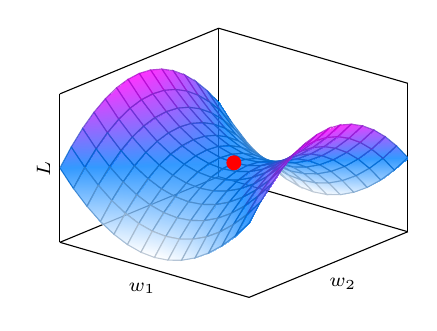
\begin{tikzpicture}
\begin{axis}[
  width=6cm, height=5cm, view={40}{30},
  xlabel={$w_1$}, ylabel={$w_2$}, zlabel={$L$},
  xtick=\empty, ytick=\empty, ztick=\empty,
  label style={font=\scriptsize},
  colormap/cool,
]
\addplot3[surf, shader=faceted interp, opacity=0.8, domain=-1:1,
  y domain=-1:1, samples=15] {x^2 - y^2};
\addplot3[only marks, mark=*, mark size=2.5pt, red] coordinates {(0,0,0)};
\end{axis}
\end{tikzpicture}}}

\vspace{2pt}
{\scriptsize Saddle point: $\nabla L = 0$ (red), yet still downhill in
some directions.}
\end{column}
\end{columns}

\end{frame}
%%%%%%%%%%%%%%%%%%%%%%%%%%%%%%%%%%%%%%%%%%%%%%%%%%%%%%%%%%%%%%%%%%%%%%
\begin{frame}[fragile]
\frametitle{Error backpropagation: computing $\nabla L$ efficiently}

\begin{itemize}
\item A network can easily have $W$ = thousands (or billions) of weights.
  % \textbf{Naive}: perturb each weight one at a time and re-run the network:
  % $W \times O(W) = O(W^2)$, infeasible.
\item[$\Rightarrow$] \textbf{Error backpropagation}: the \textbf{chain rule}
  computes \emph{every} derivative exactly, at a cost proportional to the
  number of weights, $O(W)$ (one forward $+$ one backward pass).
\end{itemize}

\vspace{4pt}
\begin{itemize}
\item Losses from maximum likelihood with i.i.d.\ data are a \textbf{sum
  over data points}:
\[
L(\bs{w}) = \sum_{n=1}^{N} L_n(\bs{w})
\]
\item So we only need $\nabla L_n$ for \textbf{one data point} $n$: use it
  directly for SGD, or sum over $n$ for batch gradient descent.
\end{itemize}

\vspace{4pt}
{\scriptsize Following Bishop, \emph{PRML} (2006), \S5.3.1}

\end{frame}
%%%%%%%%%%%%%%%%%%%%%%%%%%%%%%%%%%%%%%%%%%%%%%%%%%%%%%%%%%%%%%%%%%%%%%
\begin{frame}[fragile]
\frametitle{A general network: error signals $\delta$}

\small
\centerline{\resizebox{0.78\textwidth}{!}{%
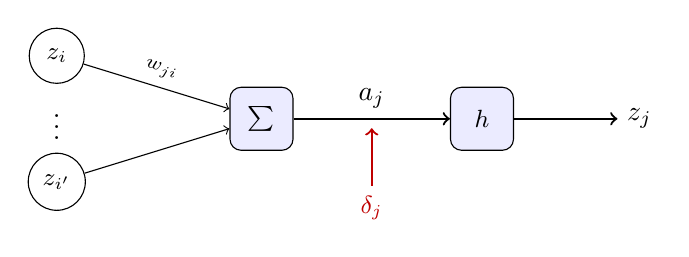
\begin{tikzpicture}[
  inp/.style={draw,circle,minimum size=0.7cm,font=\small},
  op/.style={draw,rounded corners,minimum size=0.8cm,font=\small,fill=blue!8}]
  \node[inp] (x1) at (0,0.8) {$z_i$};
  \node at (0,0.0) {$\vdots$};
  \node[inp] (xD) at (0,-0.8) {$z_{i'}$};
  \node[op] (sum) at (2.6,0) {$\sum$};
  \node[op] (h) at (5.4,0) {$h$};
  \node (z) at (7.4,0) {$z_j$};
  \draw[->] (x1) -- node[above,font=\scriptsize,sloped]{$w_{ji}$} (sum);
  \draw[->] (xD) -- (sum);
  \draw[->,thick] (sum) -- node[above]{$a_j$} (h);
  \draw[->,thick] (h) -- (z);
  \draw[red!75!black,thick,->] (4.0,-0.85) node[below,font=\small]{$\delta_j$} -- (4.0,-0.12);
\end{tikzpicture}}}

\begin{itemize}
\item Each unit: $a_j = \sum_i w_{ji} z_i$, \ $z_j = h(a_j)$,
  where $z_i$ is an input or another unit (bias: $z = 1$). Applying these
  in turn is \textbf{forward propagation}.
\item $L_n$ depends on $w_{ji}$ only via $a_j$, so by the chain rule, with the
  \textbf{error} $\delta_j \equiv \partial L_n/\partial a_j$ and
  $\partial a_j/\partial w_{ji} = z_i$:
\[
\frac{\partial L_n}{\partial w_{ji}} = \frac{\partial L_n}{\partial a_j}\,
\frac{\partial a_j}{\partial w_{ji}} = \delta_j\, z_i
\]
  $\delta$ at the output end of the link $\times$ $z$ at its input end.
\end{itemize}

\end{frame}
%%%%%%%%%%%%%%%%%%%%%%%%%%%%%%%%%%%%%%%%%%%%%%%%%%%%%%%%%%%%%%%%%%%%%%
\begin{frame}[fragile]
\frametitle{Hidden units: backpropagating the $\delta$'s}

\begin{columns}[c]
\begin{column}{0.4\textwidth}
\centerline{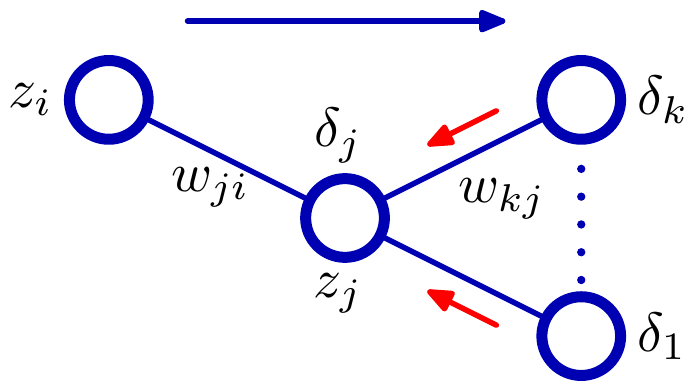
\includegraphics[width=\linewidth]{figures/prml_fig5_7.png}}

\vspace{2pt}
{\scriptsize Bishop, \emph{PRML} (2006), Fig.\ 5.7: blue, forward
propagation; {\color{red}red}, backward propagation of the errors.}
\end{column}
\begin{column}{0.57\textwidth}
\begin{itemize}
\item Unit $j$ affects $L_n$ only via the units $k$ it sends connections
  to, so sum over them:
\[
\delta_j \equiv \frac{\partial L_n}{\partial a_j}
= \sum_k \frac{\partial L_n}{\partial a_k}\,\frac{\partial a_k}{\partial a_j}
\]
\item Using $a_k = \sum_j w_{kj} z_j$ and $z_j = h(a_j)$, the \textbf{backpropagation formula}:
\[
\delta_j = h'(a_j) \sum_k w_{kj}\, \delta_k
\]
\end{itemize}
\end{column}
\end{columns}

\vspace{4pt}
\visible<2->{%
\begin{itemize}
\item For the \textbf{output} units, e.g.\ sum-of-squares loss with
  identity output: $\delta_k = y_k - t_k$.
\item[$\Rightarrow$] Start from the outputs' $\delta_k$ and apply this
  recursively: every hidden unit's $\delta$, for any feed-forward network.
\item[$\Rightarrow$] \textbf{Key idea}: compute $\delta$ once at each unit, then
  reuse it for all of that unit's incoming weights.
\end{itemize}}

\end{frame}
%%%%%%%%%%%%%%%%%%%%%%%%%%%%%%%%%%%%%%%%%%%%%%%%%%%%%%%%%%%%%%%%%%%%%%
\begin{frame}[fragile]
\frametitle{Try it: the chain rule}
\setbeamertemplate{blocks}[rounded]
\setbeamercolor{block title}{bg=orange!25,fg=black}
\setbeamercolor{block body}{bg=orange!7,fg=black}

\centerline{\resizebox{0.9\textwidth}{!}{%
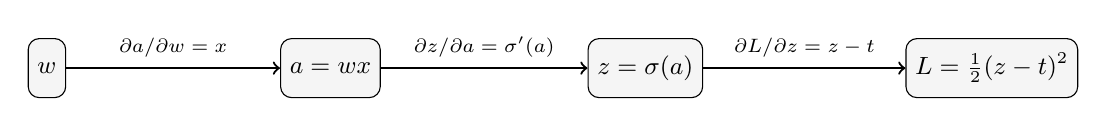
\begin{tikzpicture}[
  nd/.style={draw,rounded corners,minimum height=0.75cm,font=\small,fill=gray!8}]
  \node[nd] (w) at (0,0) {$w$};
  \node[nd] (a) at (3.6,0) {$a = wx$};
  \node[nd] (z) at (7.6,0) {$z = \sigma(a)$};
  \node[nd] (L) at (12,0) {$L = \tfrac12 (z - t)^2$};
  \draw[->,thick] (w) -- node[above,font=\scriptsize]{$\partial a/\partial w = x$} (a);
  \draw[->,thick] (a) -- node[above,font=\scriptsize]{$\partial z/\partial a = \sigma'(a)$} (z);
  \draw[->,thick] (z) -- node[above,font=\scriptsize]{$\partial L/\partial z = z - t$} (L);
\end{tikzpicture}}}

\vspace{4pt}
\begin{itemize}
\small
\item \textbf{Chain rule}: multiply the local derivatives along the path,
  \ $\partial L/\partial w = (\partial L/\partial z)\,(\partial z/\partial a)\,
  (\partial a/\partial w)$.
\end{itemize}

\begin{block}{Try it (2 min)}
With $w = 0$, $x = 2$, $t = 1$: compute $a$, $z$, $L$, then
$\partial L/\partial w$. \ (Hint: $\sigma'(a) = \sigma(a)\bigl(1-\sigma(a)\bigr)$.)
\end{block}

\visible<2->{%
\begin{itemize}
\small
\item[] $a = 0$, \ $z = \sigma(0) = 0.5$, \ $L = 0.125$, and
\[
\frac{\partial L}{\partial w} = (z - t)\,\sigma'(a)\,x = (-0.5)(0.25)(2) = -0.25
\]
  negative, so increasing $w$ lowers $L$.
\end{itemize}}

\end{frame}
%%%%%%%%%%%%%%%%%%%%%%%%%%%%%%%%%%%%%%%%%%%%%%%%%%%%%%%%%%%%%%%%%%%%%%
\begin{frame}[fragile]
\frametitle{Backpropagation: the algorithm}

\centerline{\resizebox{0.9\textwidth}{!}{%
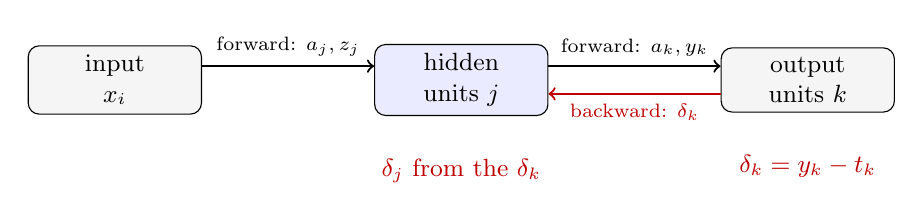
\begin{tikzpicture}[
  lay/.style={draw,rounded corners,minimum width=2.2cm,minimum height=0.75cm,
    font=\small, fill=gray!8, align=center},
  fw/.style={->,thick},
  bw/.style={->,thick,red!75!black},
  lab/.style={font=\scriptsize}]
  \node[lay] (L0) at (0,0) {input\\$x_i$};
  \node[lay,fill=blue!8] (Lj) at (4.4,0) {hidden\\units $j$};
  \node[lay] (Lk) at (8.8,0) {output\\units $k$};
  \draw[fw] ([yshift=5pt]L0.east) -- node[above,lab]{forward: $a_j, z_j$} ([yshift=5pt]Lj.west);
  \draw[fw] ([yshift=5pt]Lj.east) -- node[above,lab]{forward: $a_k, y_k$} ([yshift=5pt]Lk.west);
  \draw[bw] ([yshift=-5pt]Lk.west) -- node[below,lab]{backward: $\delta_k$} ([yshift=-5pt]Lj.east);
  \node[font=\small,text=red!75!black,below=12pt of Lk] {$\delta_k = y_k - t_k$};
  \node[font=\small,text=red!75!black,below=12pt of Lj] {$\delta_j$ from the $\delta_k$};
\end{tikzpicture}}}

\vspace{8pt}
\setbeamertemplate{blocks}[rounded]
\setbeamercolor{block title}{bg=blue!15,fg=black}
\setbeamercolor{block body}{bg=blue!4,fg=black}
\begin{block}{Error backpropagation, for each data point $(\bs{x}_n, \bs{t}_n)$}
\renewcommand{\arraystretch}{1.5}
\begin{tabular}{@{}l@{\hspace{10pt}}l@{}}
1.\ \textbf{Forward propagate} & $a_j = \sum_i w_{ji}\, z_i, \quad z_j = h(a_j)$ \ {\scriptsize\color{gray} every unit}\\
2.\ \textbf{Output errors} & $\delta_k = y_k - t_k$ \ {\scriptsize\color{gray} squared loss $+$ identity output}\\
3.\ \textbf{Backpropagate} & $\delta_j = h'(a_j) \sum_k w_{kj}\, \delta_k$ \ {\scriptsize\color{gray} deeper nets: repeat layer by layer}\\
4.\ \textbf{Derivatives} & $\partial L_n / \partial w_{ji} = \delta_j\, z_i$ \ {\scriptsize\color{gray} every weight}
\end{tabular}
\end{block}

\vspace{6pt}
\begin{itemize}
\item Batch methods: sum over data points,
  $\partial L/\partial w_{ji} = \sum_n \partial L_n/\partial w_{ji}$.
\item[$\Rightarrow$] Then take a (S)GD step; this \emph{is} how every
  network in this unit is trained.
\end{itemize}

\end{frame}
%%%%%%%%%%%%%%%%%%%%%%%%%%%%%%%%%%%%%%%%%%%%%%%%%%%%%%%%%%%%%%%%%%%%%%
% \begin{frame}[fragile]
% \frametitle{Try it: backpropagation by hand}

% \centerline{%
% \begin{tikzpicture}[
%   nd/.style={draw,circle,minimum size=0.9cm,font=\small}]
%   \node[nd] (x) at (0,0) {$x$};
%   \node[nd,fill=blue!8] (z) at (3,0) {$z$};
%   \node[nd] (y) at (6,0) {$y$};
%   \draw[->] (x) -- node[above,font=\small]{$w^{(1)}$} (z);
%   \draw[->] (z) -- node[above,font=\small]{$w^{(2)}$} (y);
%   \node[below=2pt of z,font=\scriptsize] {ReLU $h$};
%   \node[below=2pt of y,font=\scriptsize] {identity $f$};
% \end{tikzpicture}}

% \vspace{6pt}
% \begin{itemize}
% \item Tiny network, no biases: $x = 2$, target $t = 1$, weights
%   $w^{(1)} = 0.5$, $w^{(2)} = 3$; loss $L_n = \frac12 (y - t)^2$.
% \item Compute, using the formulas above:
%   \begin{enumerate}
%   \item \textbf{Forward pass}: $a$, $z$, $y$ and $L_n$
%   \item \textbf{Backward pass}: $\delta_k$ and $\delta_j$
%   \item \textbf{Gradients}: $\partial L_n/\partial w^{(2)}$ and
%     $\partial L_n/\partial w^{(1)}$
%   \item One SGD step with $\eta = 0.01$: does $L_n$ go down?
%   \end{enumerate}
% \item[$\Rightarrow$] Try it on paper; the next slide checks your gradients
%   with PyTorch.
% \end{itemize}

% \end{frame}
% %%%%%%%%%%%%%%%%%%%%%%%%%%%%%%%%%%%%%%%%%%%%%%%%%%%%%%%%%%%%%%%%%%%%%%
% \begin{frame}[fragile]
% \frametitle{Backpropagation: a worked example}

% \small
% \begin{itemize}
% \item[] $x = 2$, $t = 1$, $w^{(1)} = 0.5$, $w^{(2)} = 3$, ReLU hidden unit,
%   identity output, $L_n = \frac12(y-t)^2$.
% \end{itemize}

% \begin{enumerate}
% \uncover<2->{\item \textbf{Forward}: $a = w^{(1)}x = 1$, \ $z = \max(0,1) = 1$,
%   \ $y = w^{(2)}z = 3$, \ $L_n = \frac12(3-1)^2 = 2$}
% \uncover<3->{\item \textbf{Backward}: $\delta_k = y - t = 2$, \
%   $\delta_j = h'(a)\,w^{(2)}\delta_k = 1\cdot 3\cdot 2 = 6$ \
%   (ReLU: $h'(a) = 1$ since $a>0$)}
% \uncover<4->{\item \textbf{Gradients}: $\dfrac{\partial L_n}{\partial w^{(2)}}
%   = \delta_k z = 2$, \quad $\dfrac{\partial L_n}{\partial w^{(1)}} =
%   \delta_j x = 12$}
% \uncover<5->{\item \textbf{SGD step}: $w^{(1)} \leftarrow 0.5 - 0.01\cdot 12 =
%   0.38$, \ $w^{(2)} \leftarrow 3 - 0.01\cdot 2 = 2.98$}
% \end{enumerate}

% \vspace{4pt}
% \uncover<6->{\begin{itemize}
% \item[$\Rightarrow$] New prediction $y = 2.98\cdot\max(0, 0.76) \approx
%   2.26$, so $L_n \approx 0.80 < 2$: the step reduced the loss.
% \end{itemize}}

% \end{frame}
%%%%%%%%%%%%%%%%%%%%%%%%%%%%%%%%%%%%%%%%%%%%%%%%%%%%%%%%%%%%%%%%%%%%%%
\begin{frame}[fragile]
\frametitle{Backpropagation in PyTorch: autograd}

\begin{itemize}
\item In practice we do not need to code the backward pass by hand: frameworks
  such as \textbf{PyTorch} record the forward computation and apply the
  chain rule automatically (\textbf{autograd}).
\item The worked example, in a few lines:
\end{itemize}

\begin{lstlisting}
import torch
w1 = torch.tensor(0.5, requires_grad=True)   # track gradients
w2 = torch.tensor(3.0, requires_grad=True)
x, t = torch.tensor(2.0), torch.tensor(1.0)

y = w2 * torch.relu(w1 * x)                  # forward pass
loss = 0.5 * (y - t) ** 2                    # L_n = 2
loss.backward()                              # backpropagation
print(w1.grad, w2.grad)                      # tensor(12.) tensor(2.)
\end{lstlisting}

% \begin{itemize}
% \item[$\Rightarrow$] Answers to the exercise: $\partial L_n/\partial w^{(1)} = 12$,
%   $\partial L_n/\partial w^{(2)} = 2$; one SGD step ($\eta = 0.01$) lowers
%   $L_n$ from 2 to about 0.80.
% \end{itemize}

\end{frame}
%%%%%%%%%%%%%%%%%%%%%%%%%%%%%%%%%%%%%%%%%%%%%%%%%%%%%%%%%%%%%%%%%%%%%%
\begin{frame}[fragile]
\frametitle{Training a network in PyTorch}

\begin{lstlisting}
from torch import nn
model = nn.Sequential(nn.Linear(D, M), nn.ReLU(),   # hidden layer, h = ReLU
                      nn.Linear(M, K))               # output layer, f = identity
loss_fn = nn.MSELoss()             # mean squared error
# classification: nn.BCEWithLogitsLoss(), which applies the sigmoid itself
opt = torch.optim.SGD(model.parameters(), lr=0.01)   # eta = 0.01

for epoch in range(n_epochs):      # repeat for several epochs
    for xb, tb in loader:          # mini-batches, shuffled each epoch
        y = model(xb)              # forward pass
        loss = loss_fn(y, tb)
        opt.zero_grad()            # clear old gradients
        loss.backward()            # backpropagation: all dL/dw
        opt.step()                 # SGD update: w <- w - eta * grad
\end{lstlisting}

\begin{itemize}
\item Sizes \texttt{D, M, K}, the mini-batch \texttt{loader} and
  \texttt{n\_epochs} are set up beforehand.
\item[$\Rightarrow$] The \texttt{model}, the loss and the optimiser can change (e.g.\
  \texttt{torch.optim.Adam}).
\end{itemize}

\end{frame}
%%%%%%%%%%%%%%%%%%%%%%%%%%%%%%%%%%%%%%%%%%%%%%%%%%%%%%%%%%%%%%%%%%%%%%
\begin{titledslide}{Reading}

  \begin{itemize}
  \item Bishop, C.\,M., \emph{Pattern Recognition and Machine Learning}
    (2006), Chapter 5:
    \S5.1 (feed-forward network functions), \S5.2
    (network training, \S5.2.4 gradient descent), \S5.3 (error
    backpropagation).
    \href{https://www.microsoft.com/en-us/research/uploads/prod/2006/01/Bishop-Pattern-Recognition-and-Machine-Learning-2006.pdf}{Free
    online}.
  \item Goodfellow, Bengio, Courville, \emph{Deep Learning} (2016), Chapters
    6 and 8, a more modern treatment (ReLU, Adam, and optimisation for deep
    nets). \href{https://www.deeplearningbook.org/}{Free online} (optional,
    further reading).
  \end{itemize}

\end{titledslide}
%%%%%%%%%%%%%%%%%%%%%%%%%%%%%%%%%%%%%%%%%%%%%%%%%%%%%%%%%%%%%%%%%%%%%%
\end{document}
